% Created 2020-05-05 Tue 16:42
% Intended LaTeX compiler: pdflatex
\documentclass[11pt]{article}
\usepackage[utf8]{inputenc}
\usepackage[T1]{fontenc}
\usepackage{graphicx}
\usepackage{grffile}
\usepackage{longtable}
\usepackage{wrapfig}
\usepackage{rotating}
\usepackage[normalem]{ulem}
\usepackage{amsmath}
\usepackage{textcomp}
\usepackage{amssymb}
\usepackage{capt-of}
\usepackage{hyperref}
\usepackage{minted}
\usepackage{/home/ryan/Dropbox/profiles/Templates/LaTeX/ScreenStyle}
\usepackage[citestyle=numeric, bibstyle=numeric,hyperref=true,backref=true, maxcitenames=3,url=true,backend=biber,natbib=true]{biblatex}
\addbibresource{/home/ryan/Dropbox/Studies/Papers/references.bib}
%%% TeX-command-extra-options: "-shell-escape"
\author{Ryan Greenup}
\date{\today}
\title{Analysing Twitter for Ubisoft}
\hypersetup{
 pdfauthor={Ryan Greenup},
 pdftitle={Analysing Twitter for Ubisoft},
 pdfkeywords={},
 pdfsubject={},
 pdfcreator={Emacs 27.0.91 (Org mode 9.4)}, 
 pdflang={English}}
\begin{document}

\maketitle
\tableofcontents




\section{8.1 Analysing the Relationship Between Friends and Followers for Twitter Users}
\label{sec:orgf9610a4}
\subsection{8.1.1 Retrieve the posts from Twitter}
\label{sec:orgccb5de0}
relevant posts can be retrieved from twitter by utilising the \texttt{rtweet} package, packages can be loaded for use in \textbf{\textbf{\uline{R}}} thusly:

\begin{listing}[htbp]
\begin{minted}[]{r}
# Load Packages -----------------------------------------------------------
setwd("~/Dropbox/Notes/DataSci/Social_Web_Analytics/SWA-Project/scripts/")

if (require("pacman")) {
  library(pacman)
} else{
  install.packages("pacman")
  library(pacman)
}

pacman::p_load(xts, sp, gstat, ggplot2, rmarkdown, reshape2,
               ggmap, parallel, dplyr, plotly, tidyverse,
               reticulate, UsingR, Rmpfr, swirl, corrplot,
               gridExtra, mise, latex2exp, tree, rpart,
               lattice, coin, primes, epitools, maps, clipr,
               ggmap, twitteR, ROAuth, tm, rtweet, base64enc,
               httpuv, SnowballC, RColorBrewer, wordcloud,
               ggwordcloud, tidyverse, boot)
\end{minted}
\caption{\label{org07d73aa}Load the Packages for \textbf{\textbf{\emph{R}}}}
\end{listing}


The \texttt{rtweet} API will search for tweets that contain all the words of a query
regardless of uppercase or lowercase usage \cite{kearney2019}.

In order to leverage the \emph{Twitter} API it is necessary to use tokens provided through a \emph{Twitter} developer account:

\begin{listing}[htbp]
\begin{minted}[]{r}
# Set up Tokens ===========================================================

options(RCurlOptions = list(
  verbose = FALSE,
  capath = system.file("CurlSSL", "cacert.pem", package = "RCurl"),
  ssl.verifypeer = FALSE
))

setup_twitter_oauth(
  consumer_key = "*************************",
  consumer_secret = "**************************************************",
  access_token = "**************************************************",
  access_secret = "*********************************************"
)

# rtweet ==================================================================
tk <-    rtweet::create_token(
  app = "SWA",
  consumer_key    = "*************************",
  consumer_secret = "**************************************************",
  access_token    = "**************************************************",
  access_secret   = "*********************************************",
  set_renv        = FALSE
\end{minted}
\caption{\label{orga8fb6a4}Import the twitter tokens (redacted)}
\end{listing}

and hence all tweets containing a mention of \emph{Ubisoft} can be returned and saved to disk as shown in listing \ref{orgccbed0b}:

\begin{listing}[htbp]
\begin{minted}[]{r}
 n <- 1000
 tweets.company <- search_tweets(q = 'ubisoft', n = n, token = tk,
                                 include_rts = FALSE)
 save(tweets.company[,], file = "resources/Download_1.Rdata")
\end{minted}
\caption{\label{orgccbed0b}Save the Tweets to the HDD as an \texttt{rdata} file}
\end{listing}

\subsection{8.2.2 Count of Followers and Friends}
\label{sec:org778bc00}
In order to identify the number of users that are contained in the \emph{tweets} the
\texttt{unique()} function can be used to return a vector of names which can then be passed as an index to the vector of counts as shown in listing \ref{orgd1cc3b8}, this provides that 81.7\% of the tweets are by unique users.

\begin{listing}[htbp]
\begin{minted}[]{r}
(users <- unique(tweets.company$name)) %>% length()
x <- tweets.company$followers_count[duplicated(tweets.company$name)]
y <- tweets.company$friends_count[duplicated(tweets.company$name)]

## > [1] 817
\end{minted}
\caption{\label{orgd1cc3b8}Return follower count of twitter posts}
\end{listing}


\subsection{8.1.3 Summary Statistics}
\label{sec:org0b44c4f}
The average number of friends and followers from users who posted tweets mentioning \emph{Ubisoft} can be returned using the \texttt{mean()} as shown in listing \ref{org4329f53}
this provides that on average each user has 586 friends and 63,620 followers.

\begin{listing}[htbp]
\begin{minted}[]{r}
x<- rnorm(090)
y<- rnorm(090)
(xbar <- mean(x))
(ybar <- mean(y))

## > [1] 4295.195
## > [1] 435.9449
\end{minted}
\caption{\label{org4329f53}Determine the average number of friends and followers}
\end{listing}

\subsection{8.1.4 Above Average Followers}
\label{sec:org2ee1e56}
Each user can be compared to the average number of followers, by using a logical
operator on the vector (e.g. \texttt{y > ybar}), this will return an output of logical
values. \textbf{\emph{R}} will coerce logicals into 1/0 values meaning that the mean value
will return the proportion of \texttt{TRUE} responses as shown in listing \ref{orgab9ab28}. This
provides that:

\begin{itemize}
\item 2.4\%  of the have identified have an above average \textbf{number of followers}.
\item 20.6\% of the users identified have an above average \textbf{number of friends}.
\end{itemize}

\begin{listing}[htbp]
\begin{minted}[]{r}
(px_hat <- mean(x>xbar))
(py_hat <- mean(y>ybar))

## > [1] 0.0244798
## > [1] 0.2729498
\end{minted}
\caption{\label{orgab9ab28}Calculate the proportion of users with above average follower counts}
\end{listing}


\subsection{8.1.5 Bootstrap confidence intervals}
\label{sec:org9fc45bc}
\subsubsection{a/b.) Generate a bootsrap distribution}
\label{sec:orgfd05ef2}

A bootstrap assumes that the population is an infinitely large repetition of the
sample and may be produces with respect to follower counts by resampling with
replacement/repetition and plotted using the \texttt{ggplot2} library as deomonstrated
in listings \ref{orgb38c014} and \ref{org61957b0} and shown in figure \ref{fig:org89570b2}.

This shows that the population follower counts is a non-normal skew-right
distribution, which is expected because the number of friends is an integer value bound by zero \cite{nist2013}.

\begin{listing}[htbp]
\begin{minted}[]{r}
## Resample the Data
(bt_pop <- sample(x, size = 10^6, replace = TRUE)) %>% head()

## > [1]   7 515 262 309 186 166
\end{minted}
\caption{\label{orgb38c014}Bootstrapping a population from the sample.}
\end{listing}

\begin{listing}[htbp]
\begin{minted}[]{r}
## Make the Population
bt_pop_data <- tibble("Followers" = bt_pop)
ggplot(data = bt_pop_data, aes(x = Followers)) +
  geom_histogram(aes(y = ..density..), fill = "lightblue", bins = 35, col = "pink") +
  geom_density(col = "violetred2") +
  scale_x_continuous(limits = c(1, 800)) +
  theme_bw() +
  labs(x = "Number of Followers", y = "Density",
       title = "Bootstrapped population of Follower Numbers")

\end{minted}
\label{org61957b0}
\end{listing}

\begin{figure}[htbp]
\centering
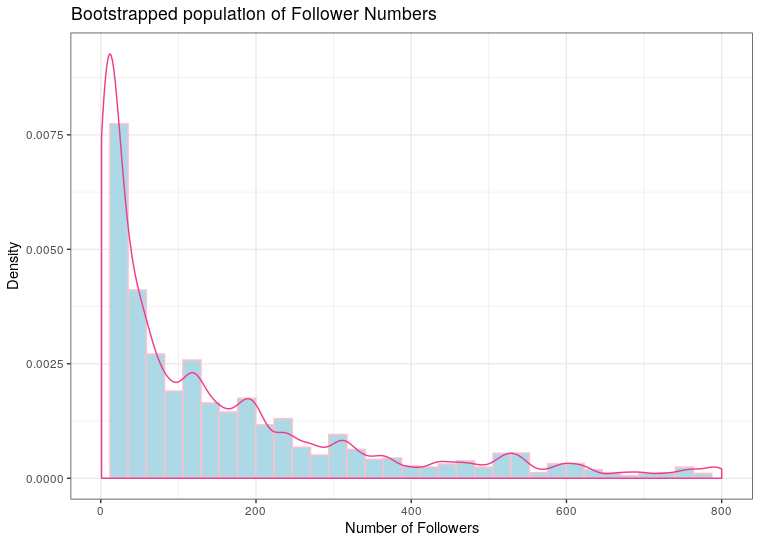
\includegraphics[width=12cm]{./Figures/BootStrap_Pop.png}
\caption{\label{fig:org89570b2}Histogram of the bootrapped population of follower counts}
\end{figure}

\subsubsection{c.) Estimate a Confidence Interval for the population mean Follower Counts}
\label{sec:orga5f0493}
In order to perform a bootrap for the population mean value of follower counts it is necessary to:

\begin{enumerate}
\item Resample the data with replacement
\begin{itemize}
\item i.e. randomly select values from the sample allowing for repetition
\end{itemize}
\item Measure the statistic of concern
\item Replicate this a sufficient number of times
\begin{itemize}
\item i.e. Greater than or equal to 1000 times \cite[Ch. 5]{davison1997}
\end{itemize}
\end{enumerate}

This is equivalent to drawing a sample from a population that is infinitely large and constructed of repetitions of the sample. This can be performed in \textbf{\emph{R}} as shown in listing \ref{orgf4baea6}.


\begin{listing}[htbp]
\begin{minted}[]{r}
xbar_boot_loop <- replicate(10^3, {
  s <- sample(x, replace = TRUE)
  mean(s)
  })
quantile(xbar_boot_loop, c((1-0.97)/2, (1+0.97)/2))

##       1.5%      98.5%
##   588.4189 10228.7352
\end{minted}
\caption{\label{orgf4baea6}Confidence Interval of Mean Follower Count in Population}
\end{listing}

A 97\% probability interval is such that a sample drawn from a population will contain the population mean in that interval 97\% of the time, this means that it may be concluded with a high degree of certainty that the true population mean lies between 588 and 10228.

\begin{enumerate}
\item Alternative Approaches
\label{sec:orgbec35f5}
If this data was normally distributed it may have been appropriate to consider
bootstrapping the standard error and using a \(t\) distribution, however it is more appropriate to use a
percentile interval for skewed data such as this, in saying that however this method is not considered to be very accurate in the literature and is often too narrow. \cite[Section 4.1]{hesterberg2015}

\begin{itemize}
\item It's worth noting that the normal \(t\) value bootstrap offers no advantage over
using a \(t\) distribution (other than being illustrative of bootstrapping
generally) \cite[Section 4.1]{hesterberg2015}
\end{itemize}


 The \texttt{boot} package is a bootstrapping library common among authors in the data science sphere
 \cite[p. 295]{james2013} \cite[p. 237]{wiley2019} that implements
 confidence intervals consistent with work by Davison and Hinkley
 \cite{ripley2020} in there texbook \emph{Bootstrap Methods and their Application}.
In this work it is provided that the \(BC_{a}\) method of constructing confidence
 intervals is  superior to mere percentile
 methods in terms of accuracy \cite[Ch. 5]{davison1997}, a sentiment echoed in the literature. \cite[Ch. 5]{carpenter2000,davison1997}

Such methods can be implemented in \textbf{\emph{R}} by passing a function to the the \texttt{boot} call as shown in listing \ref{orgbec3d1b}. This provides a broader interval, providing that the true confidence interval could lie between 1079 and 16227 followers.

\begin{listing}[htbp]
\begin{minted}[]{r}
xbar_boot <- boot(data = x, statistic = mean_val, R = 10^3)
boot.ci(xbar_boot, conf = 0.97, type = "bca", index = 1)

## BOOTSTRAP CONFIDENCE INTERVAL CALCULATIONS
## Based on 1000 bootstrap replicates
##
## CALL :
## boot.ci(boot.out = xbar_boot, conf = 0.97, type = "bca", index = 1)
##
## Intervals :
## Level       BCa
## 97%   ( 1079, 16227 )
## Calculations and Intervals on Original Scale
## Warning : BCa Intervals used Extreme Quantiles
## Some BCa intervals may be unstable
## Warning message:
## In norm.inter(t, adj.alpha) : extreme order statistics used as endpoints
\end{minted}
\caption{\label{orgbec3d1b}Bootstrap of population mean follower count implementing the \(BC_{a}\) method}
\end{listing}
\end{enumerate}


\subsubsection{d.) Estimate a Confidence Interval for the population mean Friend Counts}
\label{sec:org3b6fc56}
A Confidence interval for the population mean friend counts may be constructed in a like wise fashion as shown in listings \ref{org683e92f}. This provides that the 97\% confidence interval for the population mean friend count is between 384 and 502 (or 387 and 496 if the \(BC_{a}\) method used, they're quite close and so the more conservative percentile method will be accepted).

\begin{listing}[htbp]
\begin{minted}[]{r}
# d.) Estimate a Confidence Interval for the populattion mean Friend Count ===
# Using a Percentile Method #####################################################
ybar_boot_loop <- replicate(10^3, {
  s <- sample(y, replace = TRUE)
  mean(s)
  })
quantile(ybar_boot_loop, c(0.015, 0.985)

# Using BCA Method #############################################################
mean_val <- function(data, index) {
  X = data[index]
  return(mean(X))
}

xbar_boot <- boot(data = y, statistic = mean_val, R = 10^3)
boot.ci(xbar_boot, conf = 0.97, type = "bca", index = 1)


##     1.5%    98.5%
## 383.7619 501.5903
##
## BOOTSTRAP CONFIDENCE INTERVAL CALCULATIONS
## Based on 1000 bootstrap replicates
##
## CALL :
## boot.ci(boot.out = xbar_boot, conf = 0.97, type = "bca", index = 1)
##
## Intervals :
## Level       BCa
## 97%   (386.8, 496.7 )
## Calculations and Intervals on Original Scale
## Some BCa intervals may be unstable
\end{minted}
\caption{\label{org683e92f}Bootstrap of population mean follower count}
\end{listing}

\subsection{{\bfseries\sffamily FIXME} 8.1.6 Estimate a 97\% Confidence Interval for the High Friend Count Proportion}
\label{sec:org4f37de2}
In order to bootstrap a confidence interval for the proportion of users with
above average follower counts, repeteadly draw random samples from an infinitely
large population composed entirely of the sample, and record the sampled
proportion. this can be acheived by resampling the observations of above and
below as shown in listing \ref{orgcc4ffd7}.

This provides that:
\begin{itemize}
\item The 97\% confidence interval for the population proportion of users that have an above average number of friends is between 0.24 and 0.31.
\begin{itemize}
\item i.e. The probability of any given sample containing the population mean within this interval would be 97\%, although  that doesn't however mean that there is a 97\% probability that this interval contains the value, merely that we may be 97\% \emph{confident}
\end{itemize}
\end{itemize}

\begin{listing}[htbp]
\begin{minted}[]{r}
# 8.1.6 High Friend Count Proportion -------------------------------------------
prop <- factor(c("Below", "Above"))
## 1 is above average, 2 is below
py_hat_bt <- replicate(10^3, {
  rs      <- sample(c("Below", "Above"),
                    size = length(y),
                    prob = c(py_hat, 1-py_hat),
                    replace = TRUE)
isabove <- rs == "Above"
mean(isabove)
})
quantile(py_hat_bt, c(0.015, 0.985))


##      1.5%     98.5%
## 0.2399021 0.3072215
## > > > . + > > >
## BOOTSTRAP CONFIDENCE INTERVAL CALCULATIONS
## Based on 1000 bootstrap replicates
##
## CALL :
## boot.ci(boot.out = py_hat_boot, conf = 0.97, type = "bca")
##
## Intervals :
## Level       BCa
## 97%   ( 0.2399,  0.3072 )
## Calculations and Intervals on Original Scale
\end{minted}
\caption{\label{orgcc4ffd7}Bootstrap of Proportion of Friends above average}
\end{listing}
\subsection{8.1.7 Is the Number of Friends Independent to the Number of Followers}
\label{sec:org49d8ba9}
One method to determine whether or not the number of followers is independent of the number of friends is to bin the counts and determine whether or not the distribution of users across those counts is consistent with the hypothesis of independence.

\subsubsection{Bin the Follower and Friend Categories}
\label{sec:org7b8ea2a}
The counts may be binned by performing a logical interval test as shown in listing \ref{org5eea685}.

\begin{listing}[htbp]
\begin{minted}[]{r}
## Assign Categories
x_df <- data.frame(x)
x_df$cat[0       <= x_df$x & x_df$x < 100] <- "Tens"
x_df$cat[100     <= x_df$x & x_df$x < 1000] <- "Hundreds"
x_df$cat[1000    <= x_df$x & x_df$x < 2000] <- "1Thousands"
x_df$cat[2000    <= x_df$x & x_df$x < 3000] <- "2Thousands"
x_df$cat[3000    <= x_df$x & x_df$x < 4000] <- "3Thousands"
x_df$cat[4000    <= x_df$x & x_df$x < 5000] <- "4Thousands"
x_df$cat[5000    <= x_df$x & x_df$x < Inf] <- "5ThousandOrMore"

### Make a factor
x_df$cat <- factor(x_df$cat, levels = var_levels, ordered = TRUE)

### Determine Frequencies
(x_freq <- table(x_df$cat) %>% as.matrix())

## ** b) Find the Friend Count Frequency ===========================================
## Assign Categories
y_df <- data.frame(y)
y_df$cat[0       <= y_df$y & y_df$y < 100] <- "Tens"
y_df$cat[100     <= y_df$y & y_df$y < 1000] <- "Hundreds"
y_df$cat[1000    <= y_df$y & y_df$y < 2000] <- "1Thousands"
y_df$cat[2000    <= y_df$y & y_df$y < 3000] <- "2Thousands"
y_df$cat[3000    <= y_df$y & y_df$y < 4000] <- "3Thousands"
y_df$cat[4000    <= y_df$y & y_df$y < 5000] <- "4Thousands"
y_df$cat[5000    <= y_df$y & y_df$y < Inf]  <- "5ThousandOrMore"

### Make a factor
y_df$cat <- factor(y_df$cat, levels = var_levels, ordered = TRUE)

### Determine Frequencies
(y_freq <- table(y_df$cat) %>% as.matrix())
\end{minted}
\caption{\label{org5eea685}Use Logical Test to Assign observations into bins}
\end{listing}

\subsubsection{Find the Group frequency}
\label{sec:org32e7d64}
These values may be tabluated in order to count the occurence of users among these categories as shown in listing \ref{orga410134} and table \ref{tab:org6ff777d}.

\begin{listing}[htbp]
\begin{minted}[]{r}
vals <- t(cbind(x_freq, y_freq))
rownames(vals) <- c("Followers.x", "followers.y")
vals

##             Tens Hundreds 1Thousands 2Thousands 3Thousands 4Thousands
## Followers.x  421      317         39         11          9          2
## followers.y  262      476         47         15          6          9
##             5ThousandOrMore
## Followers.x              18
## followers.y               2
\end{minted}
\caption{\label{orga410134}Tabulate the binned counts for the distribution of users among among amount and status.}
\end{listing}

\begin{table}[htbp]
\caption{\label{tab:org6ff777d}Table of Binned Friend and Follower counts, transposed relative to code.}
\centering
\begin{tabular}{lrr}
 & \textbf{\textbf{\emph{Followers}}} & \textbf{\textbf{\emph{Friends}}}\\
\emph{Tens} & 421 & 262\\
\emph{Hundreds} & 317 & 476\\
\emph{1 - Thousands} & 39 & 47\\
\emph{2 - Thousands} & 11 & 15\\
\emph{3 - Thousands} & 9 & 6\\
\emph{4 - Thousands} & 2 & 9\\
\emph{5 Thousand or More} & 18 & 2\\
\end{tabular}
\end{table}

\subsubsection{Find the Expected Counts under each group and test for independence}
\label{sec:orgffb5c33}
The expected count of each cell, under the assumption that the two metrics are
independent, will be the proportion users per bracket multiplied by the number
of users in that status group. This implies that any cell will be:

\begin{itemize}
\item the product of the row sum, multiplied by the column sum divided by the number of counts.
\end{itemize}

This can be equivalently expressed as an outer product as shown in equation
\eqref{eq:1}, in \textbf{\emph{R}} this operation is denoted by the \texttt{\%o\%} operator, which is
shorthand for the \texttt{outer()} function, this and other summary statistics may be
evaluated as shown in listing \ref{org912a5d0}.

The outer product is such that:


$$
\mathbf{u} \otimes \mathbf {v} =\mathbf {u} \mathbf {v} ^{\textsf {T}}={\begin{bmatrix}u_{1}\\u_{2}\\u_{3}\\u_{4}\end{bmatrix}}{\begin{bmatrix}v_{1}&v_{2}&v_{3}\end{bmatrix}}={\begin{bmatrix}u_{1}v_{1}&u_{1}v_{2}&u_{1}v_{3}\\u_{2}v_{1}&u_{2}v_{2}&u_{2}v_{3}\\u_{3}v_{1}&u_{3}v_{2}&u_{3}v_{3}\\u_{4}v_{1}&u_{4}v_{2}&u_{4}v_{3}\end{bmatrix}}.
$$

This means the matrix of expected frequencies can be expressed as an outer product thusly:

\begin{align}
\mathbf{\vec{e}}= \frac{1}{n} \times \begin{bmatrix} \sum^{n}_{j= 1} \left[ o_{1j} \right] \\  \sum^{n}_{j= 1}
\left[ o_{2j} \right]  \\ \sum^{n}_{j= 1} \left[ o_{3j} \right]   \\
\sum^{n}_{j= 1} \left[ o_{4j} \right]  \\ \vdots  \\
\sum^{n}_{j= 1} \left[ o_{nj} \right]     \end{bmatrix}
\begin{bmatrix}  \sum^{n}_{j= 1} \left[ o_{i1}  \right] \\  \sum^{n}_{j= 1}
\left[ o_{i2}  \right] \\ \sum^{n}_{j= 1} \left[ o_{i3}  \right] \\ \cdots \\
\sum^{n}_{j= 1} \left[ o_{in}  \right]   \end{bmatrix}  ^{\mathrm{T}} \label{eq:1}
\end{align}

\begin{listing}[htbp]
\begin{minted}[]{r}
## ***** Calculate Summary Stats
n <- sum(vals)
bracket_prop <- colSums(vals) / n
metric_prop  <- rowSums(vals) / n
o <- vals
e <- rowSums(vals) %o% colSums(vals) / n
chi_obs <- sum((e-o)^2/e)
\end{minted}
\caption{\label{org912a5d0}Calculate Expected frequency of values under the assumption of independence.}
\end{listing}

\begin{enumerate}
\item Testing Independence
\label{sec:org49b88e8}
In order to test whether or not the distribution of users among brackets is
independent of being a follower or friend a \(\chi^{2}\) test may be used, this
can be evaluated from a model or simulated, in \textbf{\emph{R}}, the simulated test is
shown in listing \ref{org76a2177}, this provides a \(p\) -value < 0.0005, which means that the hypothesis of independence may be rejected with a high degree of certainty.

\begin{listing}[htbp]
\begin{minted}[]{r}
chisq.test(vals, simulate.p.value = TRUE)


## 	Pearson's Chi-squared test with simulated p-value (based on 2000
## 	replicates)
##
## data:  vals
## X-squared = 88.109, df = NA, p-value = 0.0004998
\end{minted}
\caption{\label{org76a2177}Chi-Square testing for independence between friend and follower bin categories.}
\end{listing}

\begin{enumerate}
\item From First Principles
\label{sec:orgce7a7f5}
The \(\chi^{2}\) statistic may be performed from first principles by randomly
sampling the values at the rate at which they occured, tabulating those counts, measuring the \(\chi^{2}\) -value and then repeating this many times.

Because the samples are random they must be independent and average number of
positives is hence an estimate for the \emph{FPR}, which is in turn an estimate for
the \(p\) -value. This technique is demonstrated in listing \ref{orga9ae793}, the p-value
being returned as 0.0004, this value is consistent with the value produced by
\textbf{\emph{R}}'s built in \texttt{chisq.test} function and so is accepted.

\begin{listing}[htbp]
\begin{minted}[]{r}
## ***** Create Vectors of factor levels
brackets <- unique(x_df$cat)
metrics <- c("follower", "friend")

## ***** Simulate the data Assuming H_0
## I.e. assuming that the null hypothesis is true in that
## the brackets assigned to followers are independent of the friends
## (this is a symmetric relation)

s <- replicate(10^4,{
  ## Sample the set of Metrics
  m <- sample(metrics, size = n, replace = TRUE, prob = metric_prop)

  ## Sample the set of Brackets (i.e. which performance bracket the user falls in)
  b <- sample(brackets, size = n, replace = TRUE, prob = bracket_prop)

  ## Make a table of results
  o <- table(m, b)
  o

  ## Find What the expected value would be
  e_sim <- t(colSums(e) %o% rowSums(e) / n)

  ## Calculate the Chi Stat
  chi_sim <- sum((e_sim-o)^2/e_sim)
  chi_sim

  ## Is this more extreme, i.e. would we reject null hypothesis?
  chi_sim > chi_obs

})

mean(s)

## [1] 4e-04
\end{minted}
\caption{\label{orga9ae793}Performing a \(\chi^{2}\) statistic from first principles}
\end{listing}
\end{enumerate}
\end{enumerate}
\subsubsection{{\bfseries\sffamily FIXME} Conclusion}
\label{sec:org4325332}
The \(p\) -value measures the probability of rejecting the null hypothesis when it is true, i.e. the probability of a detecting a \emph{false positive}, a very small \(p\) -value is hence good evidence that the null hypothesis should be rejected (because doing so would unlikely to be a mistake).

In saying that however the \(p\) -value is distinct from the \emph{power} statistic, which is a measure of \emph{/the probability of accepting the alternative hypothesis} when it is true, a low \(p\) -value is not a measurement of the probability of being correct.

Hence me way conclude, with a high degree of certainty, that the follower and friend counts are not independent of one another.
\section{8.2 Finding Themes in tweets}
\label{sec:orgb1419a6}
\subsection{8.2.8 Find Users with Above Average Friend Counts}
\label{sec:org49cb352}
Users with Above average Friend Counts can be identified by filtering the tweets
data frame for two conditions:

\begin{enumerate}
\item non-duplicated \texttt{user-id}
\item \texttt{friend\_count} greater than average
\end{enumerate}

This can be acheived easily using the \texttt{dplyr} package as shown in \ref{org6ec3f18}, the top 20 of these users are shown in table \ref{tab:orgddeb848} of the appendix

\begin{listing}[htbp]
\begin{minted}[]{r}
select <- dplyr::select
filter <- dplyr::filter
interested_vars <- c("user_id", "friends_count")
(friend_counts <- tweets.company %>%
  select(interested_vars) %>%
  filter(!duplicated(user_id)))

(high_friends <- friend_counts %>%
  filter(friends_count > mean(friends_count, na.rm = TRUE)))

## Export Friends List
write.csv(high_friends[order(
  high_friends$friends_count,
  decreasing = TRUE),], file = "/tmp/highfriend.csv")
\end{minted}
\caption{\label{org6ec3f18}Use \texttt{dplyr} to Filter for Users with a high Friend Count}
\end{listing}

\subsection{8.2.9 Find Users with Below Average Friend Counts}
\label{sec:org735251e}
Users with high friends may be determined by a similar method (or by taking the complement of the high friends) as shown in listing \ref{org7e36a74}, the lowest 20 of these users are shown in table \ref{tab:org41facb0} of the appendix.

\begin{listing}[htbp]
\begin{minted}[]{r}
(low_friends <- friend_counts %>%
  filter(friends_count <= mean(friends_count, na.rm = TRUE)))

 low_friends <- low_friends[order(
   low_friends$friends_count,
   decreasing = TRUE),]

## Export Users
write.csv(low_friends[order(
  low_friends$friends_count,
  decreasing = FALSE),], file = "/tmp/lowfriend.csv")
\end{minted}
\caption{\label{org7e36a74}Use \texttt{dplyr} to Filter for Users with a low Friend Count}
\end{listing}

\subsection{8.2.10 Find the \emph{Tweets} corresponding to users with high or low friend counts}
\label{sec:org5db9549}
The tweets corresponding to users with high and low friend counts can be
identified by filtering the dataframe based on the friend count and using that
to the index the tweets from the data frame \footnote{This works because the \texttt{tm} package preserves the order of the data, this can be confirmed by using a dataframe source as opposed to a vector source (e.g. in listing \ref{orgf04fc4c}) and comparing the ID's before/after transformation.}, alternatively it is possible
to test whether or not the ID of a user appears in the high or low vector
set using the \texttt{\%in\%} operator as shown in listing \ref{org28da6e9}.

\begin{listing}[htbp]
\begin{minted}[]{r}
## Method 1
friend_test <- tweets.company$friends_count > mean(tweets.company$friends_count)
tweets_high <- tweets.company$text[friend_test]
tweets_low <- tweets.company$text[!friend_test]

## Method 2                                                                 :15b5a74:
tweets_high <- tweets.company$text[tweets.company$user_id %in%  high_friends$user_id]
tweets_low  <- tweets.company$text[tweets.company$user_id %in%  low_friends$user_id]
tweets <- c(tweets_high, tweets_low)

## Mark as High or Low
tweets_low <- cbind(tweets_low, rep("Low_Friend", length(tweets_low)))
tweets_high <- cbind(tweets_high, rep("High_Friend", length(tweets_high)))
tweets <- as.data.frame(rbind(tweets_high, tweets_low))
tweets$Friend_Status  <- factor(tweets$Friend_Status)
\end{minted}
\caption{\label{org28da6e9}Identify tweets corresponding to users with high and low friend counts}
\end{listing}

\subsection{8.2.11 Clean the tweets}
\label{sec:orge5768c0}
\subsubsection{Create a Corpus Object}
\label{sec:orgbd4add9}
In order to clean the tweets it is necessary to create a corpus object as shown in listing \ref{orgf04fc4c}, it is possible to pass a dataframe source in order to include the user ID, this isn't strictly necessary however because the \texttt{tm} package preserves order when performing transformations.

\begin{listing}[htbp]
\begin{minted}[]{r}
tweet_source <- tm::VectorSource(tweets$text)
tweet_corpus <- tm::Corpus(x = tweet_source)
\end{minted}
\caption{\label{orgf04fc4c}Create a Corpus from the tweets}
\end{listing}

Next it is necessary to choose an enoding, a primary consideration of this is whether or not the use of \emph{emoji} characters will influence the model performance. There is research to suggest that Emoji's can be used as predictive features \cite{lecompte2017} and that they can improve \emph{sentiment analysis} models \cite{shiha2017} that implement a \emph{bag of words} approach. For these reasons \emph{emoji} characters will be preserved and \href{http://www.utf-8.com/}{UTF-8} implemented.

In order to encode the data as \emph{UTF-8}, the \texttt{iconv} function can be used as shown in listing \ref{orgc0cae85}.

\begin{listing}[htbp]
\begin{minted}[]{r}
encode <- function(x) {
    iconv(x, to = "UTF-8")
#    iconv(x, to = "latin1")
  #  iconv(x, to = "ASCII")
}

tweet_corpus <- tm_map(x = tweet_corpus, FUN = encode)
tweet_corpus_raw <- tweet_corpus
\end{minted}
\caption{\label{orgc0cae85}Encode the Data as UTF-8}
\end{listing}

\subsubsection{Process the tweets}
\label{sec:orgee585d1}
Before analysis the tweets should be modified to remove characters that may interfere with categorising words, this is referred to as cleaning, in particular the following should be implemented:

\begin{enumerate}
\item Remove URL's
\item Remove Usernames
\item remove numbers
\item remove punctuation
\item remove whitespace
\item case fold all characters to lower case
\item remove a set of stop words
\item reduce each word to its stem
\end{enumerate}

In particular it is important to reduce words to lower case before removing stop words otherwise an unorthodox use of capitalisation may prevent the word from being removed throughout.

The stop word \texttt{ubisoft} will also be used, this was the query term so it's expected to turn up at a very high frequency, the words \texttt{can} and \texttt{'s} also occured quite frequently and so were removed.

The cleaning can be implemented by mapping functions over the corpus, which is fundamentally a list, this can be performed via the \texttt{tm\_map} function as shown in listing \ref{org9b1bdfe}.



\begin{listing}[htbp]
\begin{minted}[]{r}
mystop <- c(stopwords(), "’s", "can", "ubisoft", "@ubisoft", "#ubisoft")# <<stphere>>

clean_corp <- function(corpus) {
  ## Remove URL's
  corpus <- tm_map(corpus,content_transformer(function(x) gsub("(f|ht)tp(s?)://\\S+","",x)))
  ## Remove Usernames
  corpus <- tm_map(corpus,content_transformer(function(x) gsub("@\\w+","",x)))
  ## Misc
  corpus <- tm_map(corpus, FUN = removeNumbers)
  corpus <- tm_map(corpus, FUN = removePunctuation)
  corpus <- tm_map(corpus, FUN = stripWhitespace)
  corpus <- tm_map(corpus, FUN = tolower)
  corpus <- tm_map(corpus, FUN = removeWords, mystop)
  ## stopwords() returns characters and is fead as second argument
  corpus <- tm_map(corpus, FUN = stemDocument)
  return(corpus)
}

tweet_corpus_clean <- clean_corp(tweet_corpus)
\end{minted}
\caption{\label{org9b1bdfe}Use the \texttt{tm\_map} function to clean the tweets}
\end{listing}

\subsection{8.2.12 Display the first two tweets before/after processing}
\label{sec:org71c2569}
The tweets can be viewed from inside the corpus by selecting with the \texttt{[} function \footnote{The \texttt{[} function is actually shorthand for \texttt{Extract()}, most things in
\textbf{\emph{R}} are functions, this is similar to \emph{LISP} and has to do with the origins of
the language, e.g. \texttt{sum(1:10) == (sum (1:10))}, also relevant see the relevant
xkcd in figure \ref{fig:org84a8c26}.} as demonstrated in listing \ref{org1a71952}, the first \emph{tweet} was rendered empty by the processing and the following two tweets were:

\begin{itemize}
\item \textbf{\emph{Pre-Processing}}
\begin{quote}
\begin{itemize}
\item ``Today was the first time in over a month that I have gone 24 hours without
checking the coronavirus death toll. Thanks \texttt{@Ubisoft}.''

\item ``@btwimskrank \texttt{@TheDivisionGame} \texttt{@UbiMassive} \texttt{@Ubisoft} \texttt{@jgerighty} \texttt{@hamishbode}
\texttt{@Tideman92} \texttt{@janeyo\_jane} \texttt{@slimjd} Very odd\ldots{} I'll even post a video about it.''
\end{itemize}
\end{quote}
\item \textbf{\emph{Post-Processing}}
\begin{quote}
\begin{itemize}
\item ``today first time month gone hour without check coronavirus death toll thank''

\item ``odd ill even post video''
\end{itemize}
\end{quote}
\end{itemize}

\begin{listing}[htbp]
\begin{minted}[]{r}
tweet_corpus_raw[[1]]$content
tweet_corpus_clean[[1]]$content
tweet_corpus_raw[[2]]$content
tweet_corpus_clean[[2]]$content
tweet_corpus_raw[[3]]$content
tweet_corpus_clean[[3]]$content
\end{minted}
\caption{\label{org1a71952}Load the Packages for \textbf{\textbf{\emph{R}}}}
\end{listing}

\subsection{8.2.13 Create a Term Document Matrix}
\label{sec:orga78e644}
\subsubsection{Apply Weighting Manually}
\label{sec:org993ecd4}
\begin{enumerate}
\item Create Term Documen Matrix
\label{sec:org5a2f188}
A term Document matrix (and it's transpose) can be constructed from a \texttt{corpus} using the
\texttt{tm:TermDocumentMatrix} function as shown in listing \ref{org9db8c55}.

\begin{listing}[htbp]
\begin{minted}[]{r}
tweet_matrix_tdm <- TermDocumentMatrix(tweet_corpus_clean)
tweet_matrix_dtm <- DocumentTermMatrix(tweet_corpus_clean)
\end{minted}
\caption{\label{org9db8c55}Load the Packages for \textbf{\textbf{\emph{R}}}}
\end{listing}

\item Apply TF-IDF Weighting
\label{sec:org2c3cfb8}
Weighted term frequency is defined as shown in equation \eqref{tfidf}, where:

\begin{itemize}
\item \(f_{d,t}\) is the frequency of a given term \(t\) in the a document \(d\)
\item \(w_{d,t}\) is the weight of a given term \(t\) in the a document \(d\)
\item \(N\) is the number of documents
\item \(f_{t}\) is the number of documents containing \(t\)
\end{itemize}

\begin{equation}\begin{aligned}
w_{d, t} &=\mathrm{TF}_{t} \times \mathrm{IDF}_{d, t} \\
&=\log _{e}\left(f_{d, t}+1\right) \log _{e}\left(\frac{N}{f_{t}}\right) \label{tfidf}
\end{aligned}\end{equation}

This would requre multiplying each term of each row of the \(\mathrm{TF}_{t}\) matrix by the corresponding vector element of \(\mathrm{IDF}_{d,t}\), this can be implemented by taking the matrix product of a diagonalised matrix, this is shown in listing \ref{org2044579}.

\begin{listing}[htbp]
\begin{minted}[]{r}
N <- nrow(as.matrix(tweet_matrix_dtm))   # Number of Documents
ft=colSums(as.matrix(tweet_matrix_dtm) > 0) #in how many documents term t appeared in,

TF <- log(as.matrix(tweet_matrix_dtm) + 1)  # built in uses log2()
IDF <- log(N/ft)

tweet_weighted           <- TF %*% diag(IDF)
colnames(tweet_weighted) <- colnames(tweet_matrix_dtm)
\end{minted}
\caption{\label{org2044579}Apply TF-IDF Weigting}
\end{listing}

There is however a function built in to the \texttt{tm} package that will weight term document matrices and this will instead be implented to analyse the data because it will produce more maintainable code.
\end{enumerate}

\subsubsection{Apply Weighting with Built in Function}
\label{sec:org3724640}
In order to create a term document matrix (and its transpose) with TF-IDF weighted values, the \texttt{weighting} argument may be specified as \texttt{weightTfIdf} by passing an appropriate list to the \texttt{control} argument of the \texttt{TermDocumentMatrix}, as shown in listing \ref{orgac8aa95}

\begin{listing}[htbp]
\begin{minted}[]{r}
tweet_weighted_tdm <- tm::TermDocumentMatrix(x = tweet_corpus_clean, control = list(weighting = weightTfIdf))
tweet_weighted_dtm <- as.DocumentTermMatrix()  %>%
                        as.matrix()
\end{minted}
\caption{\label{orgac8aa95}Create a Document Term Matrix by transforming a Term Document Matrix}
\end{listing}

\subsubsection{Remove Empty Documents}
\label{sec:org6721f66}
Empty Documents may be removed from the matrix by a logical test as shown in listing  \ref{org22bb508} \footnote{It is important not to filter based the logic of an empty vector, because
otherwise an empty vector will returned, hence the if statement in listing \ref{org22bb508}.} this provides that 328 documents were empty following the processing. A summary of the first rows and columns of this matrix, following the removal of empty documents, is provided in table \ref{tab:org36c1832} of the appendix.

\begin{listing}[htbp]
\begin{minted}[]{r}
null = which(rowSums(as.matrix(tweet_weighted_dtm)) == 0)
rowSums(as.matrix(tweet_weighted_dtm)==0)

if(length(null)!=0){
  tweet_weighted_dtm = tweet_weighted_dtm[-null,]
}

length(null)

## [1] 328
\end{minted}
\caption{\label{org22bb508}Load the Packages for \textbf{\textbf{\emph{R}}}}
\end{listing}
\subsection{8.2.14 How many Clusters are there}
\label{sec:orgb7c1130}
\subsubsection{Use Cosine Distance}
\label{sec:orgb96a7dd}
In order to consider clustering, it can be more effective to consider the distance between the weigted documents in terms of cosine distance, the cosine distance can be calculated from the euclidean distance using the identity shown in \eqref{cos}, and this can be performed in \textbf{\emph{R}} by taking the matrix product of a diagonalised matrix as shown in listing \ref{org40b0040}.

\begin{align}
\mathrm{dist}\left( \mathbf{X}, \mathbf{Y} \right)= \left| \left| \mathbf{X}-\mathbf{Y} \right| \right| \\
&= \sqrt{\sum^{n}_{i= 1}   \left[ \left( x_i-y_i \right)^2 \right] } \\
\mathrm{dist}\left( \mathbf{X}, \mathbf{Y} \right)^2&= \sum^{n}_{i= 1}  \left[ \left( x_i-y_i \right)^2 \right] \\
&= \sum^{n}_{i= 1}   \left( x^2 \right)+  \sum^{n}_{i= 1}   \left( y_i^2 \right)+ 2 \sum^{n}_{i= 1}   \left( x_iy_i \right) \\
&= 1+ 1 +  2 \times  \frac{\sum^{n}_{i= 1}   \left( x_iy_i \right)}{\left( 1 \right) }\\
&= 2+ 2\times \frac{\sum^{n}_{i= 1}   \left( x_iy_i \right)}{\left| \left| \mathbf{X} \right| \right|\times \left| \left| \mathbf{Y} \right| \right|}\\
&= 2+ 2 \cos\left( \mathbf{X}, \mathbf{Y} \right)\\
\ \\
& \implies  \left( 1- \cos\left( \mathbf{X}, \mathbf{Y} \right) \right) = \frac{\mathrm{dist}\left( \mathbf{X}, \mathbf{Y} \right)}{2} \label{cos}
\end{align}

\begin{listing}[htbp]
\begin{minted}[]{r}
norm.tweet_weighted_dtm = diag(
                    1/sqrt(rowSums(tweet_weighted_dtm^2))
                    ) %*% tweet_weighted_dtm
D =dist(norm.tweet_weighted_dtm, method = "euclidean")^2/2
\end{minted}
\caption{\label{org40b0040}Load the Packages for \textbf{\textbf{\emph{R}}}}
\end{listing}

\subsubsection{Project into Euclidean Space}
\label{sec:org6d45314}
The cosine distance however is not appropriate to perform clustering on and so instead should be projected back into euclidean space, this can be acheived using \emph{Multi-Dimensional Scaling} via the \texttt{cmdscale} functionas shown in listing \ref{org4f0022b}. The distance is a measure of between document distance so the number of dimensions should correspond to the number of documents, however, if there are zero-value eigenvalues, these dimensions won't help explain the data in the projection, hence the number of eigenvalues has been used as the dimension of projection in this case.

\begin{listing}[htbp]
\begin{minted}[]{r}
l <- min(nrow(tweet_weighted_dtm),
         ncol(tweet_weighted_dtm))
ev <- eigen(tweet_weighted_dtm[1:l, 1:l])
k <- (ev$values != 0) %>% sum()

mds.tweet_weighted_dtm <- cmdscale(D, k=k) #TODO What should K be? see issue #10
\end{minted}
\caption{\label{org4f0022b}Load the Packages for \textbf{\textbf{\emph{R}}}}
\end{listing}

\subsubsection{Measure Within Cluster Variance}
\label{sec:orgcf99138}
In order to determine the appropriate number of clusters, the within cluster
variance can be measurd, the number of clusters at which this value ceases to
decrease is indicative of a potentially appropriate number of clusters. This is
implemented in listing \ref{orgd972d90} and shown in figure \ref{fig:org1ec920b}.

\begin{listing}[htbp]
\begin{minted}[]{r}
set.seed(271)
n = 15 # Assume it bends at 7 clusters
SSW = rep(0, n)
for (a in 1:n) {
  K = kmeans(mds.tweet_weighted_dtm, a, nstart = 20)
  SSW[a] = K$tot.withinss
  paste(a*100/n, "%") %>% print()
}
SSW


SSW_tb <- tibble::enframe(SSW)
ggplot(SSW_tb, aes(x = name, y = value)) +
  geom_point(col = "#Cd5b45", size = 5) +
  geom_line(col = "#Da70d6") +
  geom_vline(xintercept = 7, lty  = 3, col = "blue") +
  theme_bw() +
  labs(x = "Number of Clusters",
       y = "Within Cluster Sum of Square Distance",
       title = "Within Cluster Variance across Clusters")
\end{minted}
\caption{\label{orgd972d90}Use a loop to evaluate the performace of various cluster models, plot this with \emph{ggplot2}}
\end{listing}

Figure \ref{fig:org1ec920b} Indicates a sudden stop of decrease in variance at 7 clusters and following that the within cluster variance begins to decrease at a slightly slower rate. For this reason 7 could be an appropriate candidate for the number of clusters, however the minimal amount of change in the within-cluster variance indicates that the data is most likely not clustered at all.


\begin{figure}[htbp]
\centering
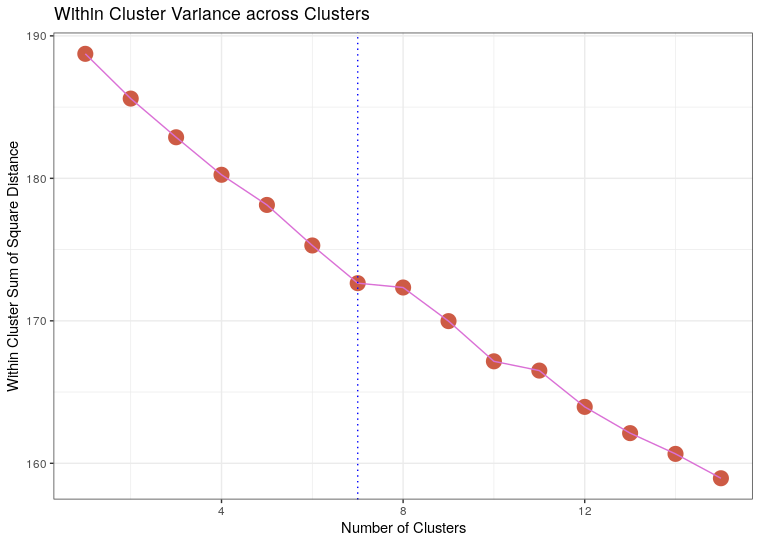
\includegraphics[width=10cm]{./Figures/Q14WithinClusterVariance.png}
\caption{\label{fig:org1ec920b}Plot of the Within Cluster Variance of the tweets using cosine distance (projected into Euclidean Space)}
\end{figure}

\subsection{8.2.15 Find the Number of tweets in each cluster}
\label{sec:org8d6c4d3}
Moving forward we'll use 3 clusters, 7 is too large and a smaller number will likely be more effective at categorising the data (particularly given that the stratification of the data appears to be quite limited from figure \ref{fig:org1ec920b}). The number of tweets in a cluster may be measured by using the \texttt{table} function as shown in listing \ref{org2715bcd} and table \ref{tab:org62d2295}.

\begin{listing}[htbp]
\begin{minted}[]{r}
K = kmeans(mds.tweet_weighted_dtm, 3, nstart = 20)
table(K$cluster)
\end{minted}
\caption{\label{org2715bcd}The \texttt{table} function can count the number of tweets per cluster.}
\end{listing}

\begin{table}[htbp]
\caption{\label{tab:org62d2295}Number of tweets in each cluster identified by \(k\) means clustering}
\centering
\begin{tabular}{lrrr}
Cluster & 1 & 2 & 3\\
\hline
\texttt{\#} of \emph{tweets} & 77 & 58 & 537\\
\end{tabular}
\end{table}

\subsection{8.2.16 Visualise the Clusters}
\label{sec:org6ece79e}
The clusters can be projected into 2D \emph{Euclidean}-Space using \emph{Multi-Dimensional
Scaling}, these dimensions would represent the first two principle components of
the cosine distance of the weigted tweets. This is demonstrated in listings
\ref{org5fb9b98}. A plot of the friend countstaus mapped to shape and clusters mapped to
colour is demonstrated in listing \ref{orgc2d778f} shown in \ref{fig:orgc57837e}, In order to get a better
understanding of the distribution of friend counts a plot of the friend count
status mapped to colour is demonstrated in listing \ref{org731750e} and shown in figure \ref{fig:orgc57837e}.


\begin{listing}[htbp]
\begin{minted}[]{r}
MDS_Euclid_2D <- cmdscale(D, k=2) #TODO What should K be? see issue #10
mds_data$Cluster       <- factor(mds_data$Cluster)

if (nrow(MDS_Euclid_2D[,1:2]) == length(K$cluster)
   && length(K$cluster) == nrow(tweets[-null,])) {
mds_data <- cbind(MDS_Euclid_2D[,1:2], "Cluster" = K$cluster, tweets[-null,])
}

mds_data$Cluster       <- factor(mds_data$Cluster)
names(mds_data)[1:2] <- c("MDS1", "MDS2")
\end{minted}
\caption{\label{org5fb9b98}Use \emph{Multi-Dimensional} scaling to project the data into 2 dimensions}
\end{listing}

\begin{listing}[htbp]
\begin{minted}[]{r}
ggplot(pca_data, aes(x = MDS1, y = MDS2, col = Friend_Status)) +
  geom_point(aes(shape = Cluster), size = 2) +
  stat_ellipse(level = 0.95) +
  theme_classic() +
  labs(main = "Principal Components of Twitter Data",
       x = TeX("MDS_1"), y = TeX("MDS_2")) +
  scale_color_discrete(label = c("High Friends", "Low Friends")) +
  guides(col = guide_legend("Friend Count \n Status"))
\end{minted}
\caption{\label{org731750e}Create a plot of the distribution of Friends among Clusters as shown in figure \ref{fig:orge2fc207}}
\end{listing}

\begin{listing}[htbp]
\begin{minted}[]{r}
ggplot(pca_data, aes(x = MDS1, y = MDS2, col = Cluster)) +
  geom_point(aes(shape = Friend_Status), size = 2) +
  stat_ellipse(level = 0.9) +
  theme_classic() +
  labs(main = "Principal Components of Twitter Data",
       x = TeX("MDS_1"), y = TeX("MDS_2")) +
  scale_shape_discrete(label = c("High Friends", "Low Friends")) +
  guides(shape = guide_legend("Friend Count \n Status"))
\end{minted}
\caption{\label{orgc2d778f}Create a plot of the distribution of Friends Count Status as shown in figure \ref{fig:orgc57837e}}
\end{listing}

\begin{figure}[htbp]
\centering
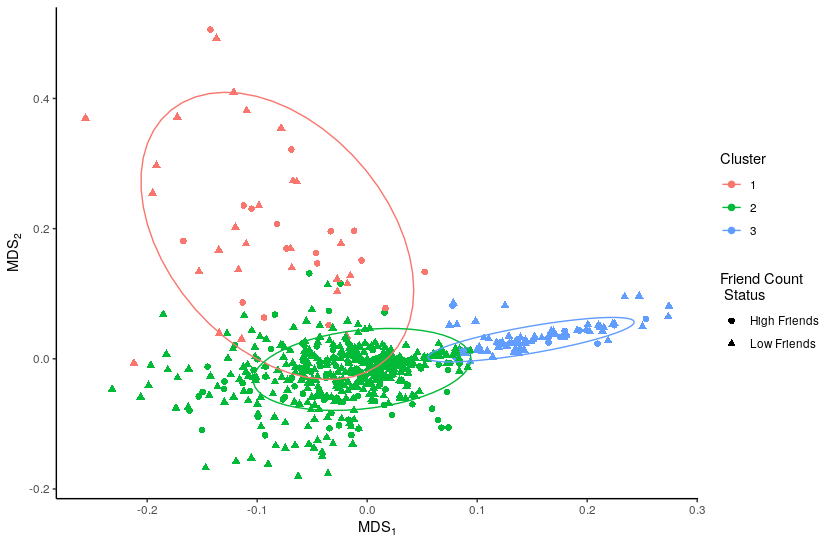
\includegraphics[width=9cm]{./Figures/betclustplot8216.png}
\caption{\label{fig:orge2fc207}Distribution of Friend Count Status over Clusters}
\end{figure}

\begin{figure}[htbp]
\centering
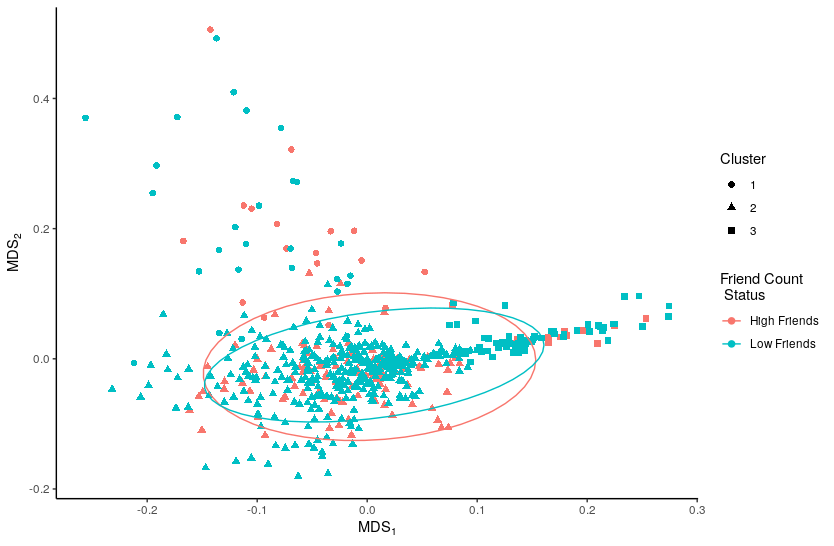
\includegraphics[width=9cm]{./Figures/betfriendplot8216.png}
\caption{\label{fig:orgc57837e}Distribution of Friend Count Status}
\end{figure}

\subsection{8.2.17 Comment on the Visualisation}
\label{sec:org1959890}
Figure \ref{fig:orge2fc207} indicates that altough there isn't a clear distinction between
clusters there is seperation of the tweets in such a way that does allow some
degree of classification to occur. Figure \ref{fig:orge2fc207} and \ref{fig:orgc57837e} both indicate that having
many or few friends is reasonably independent of the cluster that the tweet
belongs to.
\subsection{8.2.18 Cluster with Highest Number Friends}
\label{sec:org5469a94}
The Number of above or below friends corresponsing to a given cluster can be tabulated by using the \texttt{table} function as shown in listing \ref{org8a00a6c} and table \ref{tab:org623c710}, this indicates that there is a difference in the proportion of users with above average friend counts between clusters with cluster \texttt{\#1} having the highest proportion of users with above average friend counts.

\begin{listing}[htbp]
\begin{minted}[]{r}
(clust_friend <- table(
  pca_data[,names(pca_data) %in% c("Cluster", "Friend_Status")])
)

cbind(clust_friend,
        "Proportion" = signif(
            (clust_friend[,1] / rowSums(clust_friend)),
            2)
      )
\end{minted}
\caption{\label{org8a00a6c}Tabulate the distribution of friends in}
\end{listing}

\begin{table}[htbp]
\caption{\label{tab:org623c710}Above Average Friend Counts Across Clusters}
\centering
\begin{tabular}{lrrr}
\textbf{\emph{Cluster}} & \textbf{\emph{Above Average}} & \textbf{\emph{Below Average}} & \textbf{\emph{Proportion}}\\
\texttt{1} & 17 & 27 & 0.39\\
\texttt{2} & 141 & 407 & 0.26\\
\texttt{3} & 16 & 64 & 0.20\\
\end{tabular}
\end{table}

\subsection{8.2.18 Sample Tweets from cluster}
\label{sec:org6bea235}
Tweets can be sampled from the clusters by using the \texttt{sample} function with a logical test, this can be combined with a \texttt{for} loop as shown in listing \ref{org3e0a0c7}, this provides the following output.


\begin{quote}
\begin{itemize}
\item \textbf{Cluster 1}
\begin{itemize}
\item \href{https://twitter.com/search?q=\%40BelovedOfBayek\&src=typed\_query}{@BelovedOfBayek}
 \href{https://twitter.com/search?q=\%40BayekOfSiwa\&src=typed\_query}{@BayekOfSiwa} \href{https://twitter.com/search?q=\%40assassinscreed\&src=typed\_query}{@assassinscreed} \href{https://twitter.com/search?q=\%40Ubisoft\&src=typed\_query}{@Ubisoft} \href{https://twitter.com/search?q=\%40UbisoftMTL\&src=typed\_query}{@UbisoftMTL}
\href{https://twitter.com/search?q=\%40Captured\_Collec\&src=typed\_query}{@Captured\textsubscript{Collec}} \href{https://twitter.com/search?q=\%40GamerGram\_GG\&src=typed\_query}{@GamerGram\textsubscript{GG}} \href{https://twitter.com/search?q=\%40\_GameScreenshot\&src=typed\_query}{@\textsubscript{GameScreenshot}} And those smiles - and
love - are contagious. Believe me, it makes me very happy! What you have is
special! 💗 \textasciitilde{} Steffi
\item \href{https://twitter.com/search?q=\%40Ubisoft}{@Ubisoft} why is it wen I headshot sumone why don’t it register a headshot
is a 1 shot kill fix your game sir
\item \href{https://twitter.com/search?q=\%40BikiniBodhi}{@BikiniBodhi} I think we need another movement going. Obviously Ubisoft
already has plans for the next few releases of ops but we really need an Op
whose ability is to reinforce more walls than others. Especially another
castle on the team but for walls. Like 4 walls instead of 2.
\item The United Arab Emirates logged into my Ubisoft account. For why?
\item \href{https://twitter.com/search?q=\%40Atalagummy}{@Atalagummy} Está gratis este finde en lo de ubisoft creo
\end{itemize}
\item \textbf{Cluster 2}
\begin{itemize}
\item Here's everything you need to know about Ubisoft's Watch Dogs Legion in
Hindi - Release date, Story - Everything we know about it till now.
\url{https://t.co/B4lMshJdqw} via \href{https://twitter.com/search?q=\%40YouTube}{@YouTube}
\item \href{https://twitter.com/search?q=\%40Rainbow6Game}{@Rainbow6Game} \href{https://twitter.com/search?q=\%40TheGodlyNoob}{@TheGodlyNoob} I have never seen a game company ruin their
reputation so fast and so careless as Ubisoft
\item tiltei com a ubisoft, dei block na minha conta sem querer, to mt puto, real
\item My first game that really hyped me was a game called rolling thunder back in
the 80’s \url{https://t.co/mPWim2hwVY}
\item \href{https://twitter.com/search?q=\%40videogamemorals}{@videogamemorals} \href{https://twitter.com/search?q=\%40PartisanClown}{@PartisanClown} Two more remakes of Lunar: The Silver
Star, Lunar Legend and Lunar: Silver Star Harmony, were released in 2002
by Media Rings and Ubisoft and in 2009 by GungHo Online
Entertainment and Xseed Games, respectively.$\backslash$
\end{itemize}
\item \textbf{Cluster 3}
\begin{itemize}
\item \href{https://twitter.com/search?q=\%40Ubisoft}{@Ubisoft} \href{https://twitter.com/search?q=\%40UbisoftSupport}{@UbisoftSupport} crossplay between xbox and pc for Division 2
please?
\item \href{https://twitter.com/search?q=\%40tornado\_raphi}{@tornado\textsubscript{raphi}} \href{https://twitter.com/search?q=\%40Ubisoft}{@Ubisoft} \href{https://twitter.com/search?q=\%40UbisoftDE}{@UbisoftDE} Haha wollte auch einmal schlau sein
:(
\item \texttt{@Ubisoft} I was in the middle in a game waiting for us to spawn in and it
took forever and it somehow kicked me from the game for inactivity. Anyway to
fix this \url{https://t.co/Uz1yZ73R4M}
\item \href{https://twitter.com/search?q=\%40Operatedleech87}{@Operatedleech87} Yo lo veia al revez algo de Ubisoft en Girls Frontline,
pero igual un juego en consola jalaria.
\item \href{https://twitter.com/search?q=\%40VGPNetwork}{@VGPNetwork} \href{https://twitter.com/search?q=\%40GamerGram\_GG}{@GamerGram\textsubscript{GG}} \href{https://twitter.com/search?q=\%40Ubisoft}{@Ubisoft} Haha.. I love that film!
\end{itemize}
\end{itemize}
\end{quote}


\begin{listing}[htbp]
\begin{minted}[]{r}
set.seed(8923)
  for(i in 1:3) {
    n <- sample(which(pca_data$Cluster == i), size = 5)
    print(tweets$text[n])
    print("===========================")
    print("===========================")
  }
\end{minted}
\caption{\label{org3e0a0c7}Sample Tweets from the Individual Clusters}
\end{listing}

\subsection{8.2.19 Identify themes in the Tweets}
\label{sec:org96fbd23}
\subsubsection{Highest Friends Count}
\label{sec:orgc2e6e71}
The themes in the cluster with the highest friend count are:

\begin{itemize}
\item Discussion about upcoming titles
\begin{itemize}
\item For example the \emph{Sunborn-Ubisoft} collaboration
\begin{itemize}
\item This is where the use of \texttt{collab} comes from in figure \ref{fig:orgc5589c7}
\end{itemize}
\item The upcoming \emph{Division 2} release
\end{itemize}
\item Multiplayer games.
\end{itemize}
\subsubsection{Lowest Friends Count}
\label{sec:org064950f}

The themes in the cluster with the lowest friends count are:

\begin{itemize}
\item Discussion about older titles
\begin{itemize}
\item e.g. \texttt{mincemeat} refers to \emph{Farcry}, mozzi is a \emph{Rainbow 6} character
\item the recurring use of \texttt{remember} and \texttt{earliest}
\end{itemize}
\item Console games and crossplay between them
\item Feature Requests
\end{itemize}

\subsection{8.2.20 Create WordClouds}
\label{sec:org8ea4689}
Creating a wordcloud from the stemmed words will make for a poor visualisation
while creating a wordcloud based merely on the frequency of words will poorly
identify words central to the theme of the cluster.

In light of this, the most appropriate method to generate wordclouds for the
purpose visualisising the themes of the clusters is to create a document term
matrix based on a corpus cleaned without word stemming as shown in listing \ref{org74a3571}.
Following that wordclouds can then be generated by indexing for the cluster,
this is demonstrated in listing \ref{org82b7a0b} and shown in figures \ref{fig:orgc5589c7} and \ref{fig:org9874b2c}.


\begin{listing}[htbp]
\begin{minted}[]{r}
clean_corp_ns <- function(corpus) {
  ## Remove URL's
  corpus <- tm_map(corpus,content_transformer(
    function(x) gsub("(f|ht)tp(s?)://\\S+","",x)))
  ## Remove Usernames
  corpus <- tm_map(corpus,content_transformer(function(x) gsub("@\\w+","",x)))
  ## Misc
  corpus <- tm_map(corpus, FUN = removeNumbers)
  corpus <- tm_map(corpus, FUN = removePunctuation)
  corpus <- tm_map(corpus, FUN = stripWhitespace)
  corpus <- tm_map(corpus, FUN = tolower)
  corpus <- tm_map(corpus, FUN = removeWords, mystop)
  ## stopwords() returns characters and is fead as second argument
  return(corpus)
}

tweet_corpus_clean_ns <- clean_corp(tweet_corpus)

tweet_raw_dtm <- tm::TermDocumentMatrix(x = tweet_corpus_ns,
   control = list(weighting = weightTfIdf)) %>%
  as.DocumentTermMatrix()  %>%
  as.matrix()

null = which(rowSums(as.matrix(tweet_matrix_dtm)) == 0)
length(null)

(rowSums(as.matrix(tweet_matrix_dtm))) %>% table()
if(length(null)!=0){
  tweet_matrix_dtm = tweet_matrix_dtm[-null,]
}

\end{minted}
\caption{\label{org74a3571}Apply \emph{TF-IDF} weighting to an unstemmed corpus and then use a \texttt{for} loop to create wordclouds corresponding to each cluster.}
\end{listing}

\begin{listing}[htbp]
\begin{minted}[]{r}
i <- 1

for (i in c(1,3)) {
  n <- which(pca_data$Cluster == i)

  (relevant <- sort(apply(tweet_raw_dtm[n,], 2, mean),
    decreasing = TRUE)[1:30]) %>% head()

  p <- brewer.pal(n = 5, name = "Set2")
    wordcloud(
    words = names(relevant),
    freq = relevant,
    colors = p,
    random.color = FALSE
  )

}
\end{minted}
\caption{\label{org82b7a0b}Apply \emph{TF-IDF} weighting to an unstemmed corpus and then use a \texttt{for} loop to create wordclouds corresponding to each cluster.}
\end{listing}

\begin{figure}[htbp]
\centering
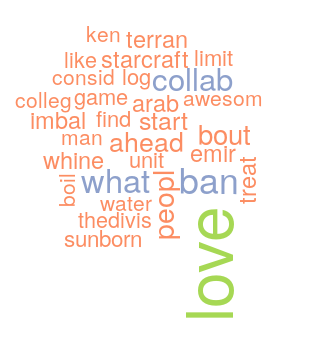
\includegraphics[width=8cm]{./Figures/Cluster1Cloud.png}
\caption{\label{fig:orgc5589c7}Wordcloud of Cluster \texttt{\#} 1 using \emph{TF-IDF} weighting}
\end{figure}

\begin{figure}[htbp]
\centering
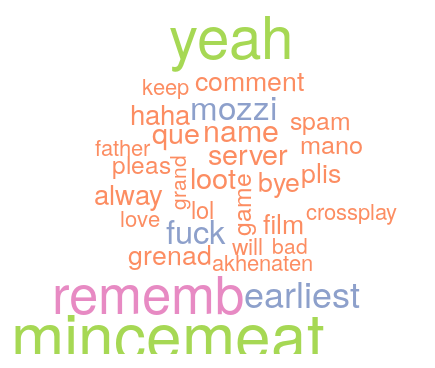
\includegraphics[width=10cm]{./Figures/Cluster3Cloud.png}
\caption{\label{fig:org9874b2c}Wordcloud of Cluster \texttt{\#} 3 using \emph{TF-IDF} weighting}
\end{figure}

\subsection{8.2.21 Use a Dendrogram to Display the Themes}
\label{sec:org25587d3}
A Dendrogram can be used to display the themes of the higest and lowest
clusters. In order to do this the most frequent words of a cluster need to be
filtered out in order to reduce the dimensions of the dendrogram, following that
a dendrogram may be made to model the cosine distance between the terms. To
acheive this in \textbf{\textbf{\uline{R}}} the identity from equation \eqref{cos} can be used and
then a dendrogram modelled over the term document matrix.


\subsubsection{Highest Friend Count}
\label{sec:org1f589b4}
Any word that occurs more than once was a candidate for the dendrogram visualising the themes of the cluster with the highest number of friends. This dendrogram is shown in figure \ref{fig:org2826cbd} and the corresponding code to produce it is provided in listing \ref{org26c7cc2}.

\subsubsection{Lowest Friend Count}
\label{sec:orga5a874a}
Any word that occurs more than once was a candidate for the dendrogram visualising the themes of the cluster with the lowest number of friends. This dendrogram is shown in figure \ref{fig:org4715ef1} and the corresponding code to produce it is provided in listing \ref{org3bf3dad}.

\begin{listing}[htbp]
\begin{minted}[]{r}
## Filter the Data To match the Cluster
tweet_weighted_dtm_c1 <- tweet_weighted_dtm[pca_data$Cluster==1, ]

## Choose terms of a given frequency to reduce the dimensions
frequent.words = which(colSums(tweet_weighted_dtm_c1 > 0) > 1)
term.matrix = tweet_weighted_dtm_c1[,frequent.words]

## In order to use the Cosine Distance Make each vector have a
## magnitude of 1
unit_term.matrix = term.matrix %*% diag(1/sqrt(colSums(term.matrix^2)))

## Preserve the column Names
colnames(unit_term.matrix) = colnames(term.matrix)
colnames(unit_term.matrix)

## Find the Cosine Distance between the Terms
## (Distance between terms so transpose)
t(unit_term.matrix)
D = dist(t(unit_term.matrix), method = "euclidean")^2/2

## Perform Heirarchical Clustering
h = hclust(D, method="average")
plot(h, main = "Themes of Cluster with Highest Friend Count")






\end{minted}
\caption{\label{org26c7cc2}Create a dendrogram of the terms in the cluster with the higest friends count, average linkage was used.}
\end{listing}

\begin{listing}[htbp]
\begin{minted}[]{r}
## Filter the Data To match the Cluster
tweet_weighted_dtm_c1 <- tweet_weighted_dtm[pca_data$Cluster==3, ]

## Choose terms of a given frequency to reduce the dimensions
frequent.words = which(colSums(tweet_weighted_dtm_c1 > 0) > 3)
term.matrix = tweet_weighted_dtm_c1[,frequent.words]

## In order to use the Cosine Distance Make each vector have a
## magnitude of 1
unit_term.matrix = term.matrix %*% diag(1/sqrt(colSums(term.matrix^2)))

## Preserve the column Names
colnames(unit_term.matrix) = colnames(term.matrix)
colnames(unit_term.matrix)

## Find the Cosine Distance between the Terms
## (Distance between terms so transpose)
t(unit_term.matrix)
D = dist(t(unit_term.matrix), method = "euclidean")^2/2

## Perform Heirarchical Clustering
h = hclust(D, method="complete")
plot(h, main = "Themes of Cluster with Lowest Friend Count")






\end{minted}
\caption{\label{org3bf3dad}Create a dendrogram of the terms in the cluster with the higest friends count, average linkage was used.}
\end{listing}


\begin{figure}[htbp]
\centering
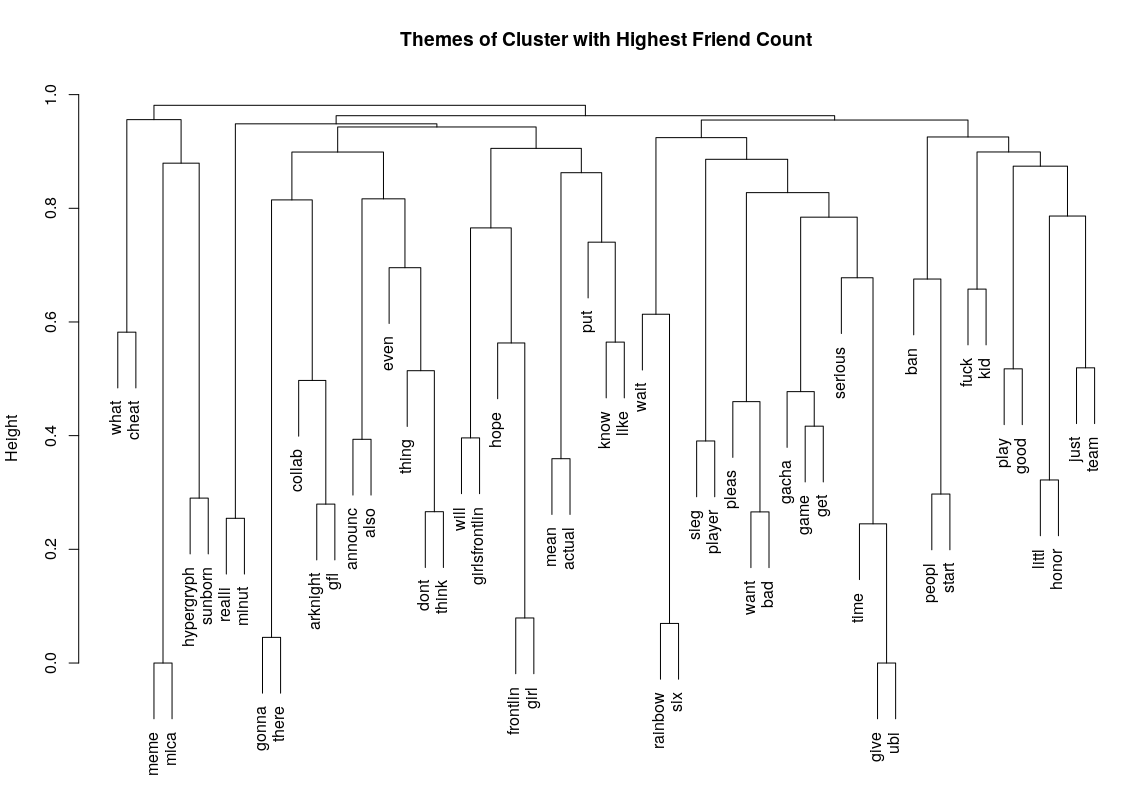
\includegraphics[width=12cm]{./Figures/HighDend.png}
\caption{\label{fig:org2826cbd}Dendrogram of Terms in the cluster with the highest friend count using average Linkage.}
\end{figure}


\begin{figure}[htbp]
\centering
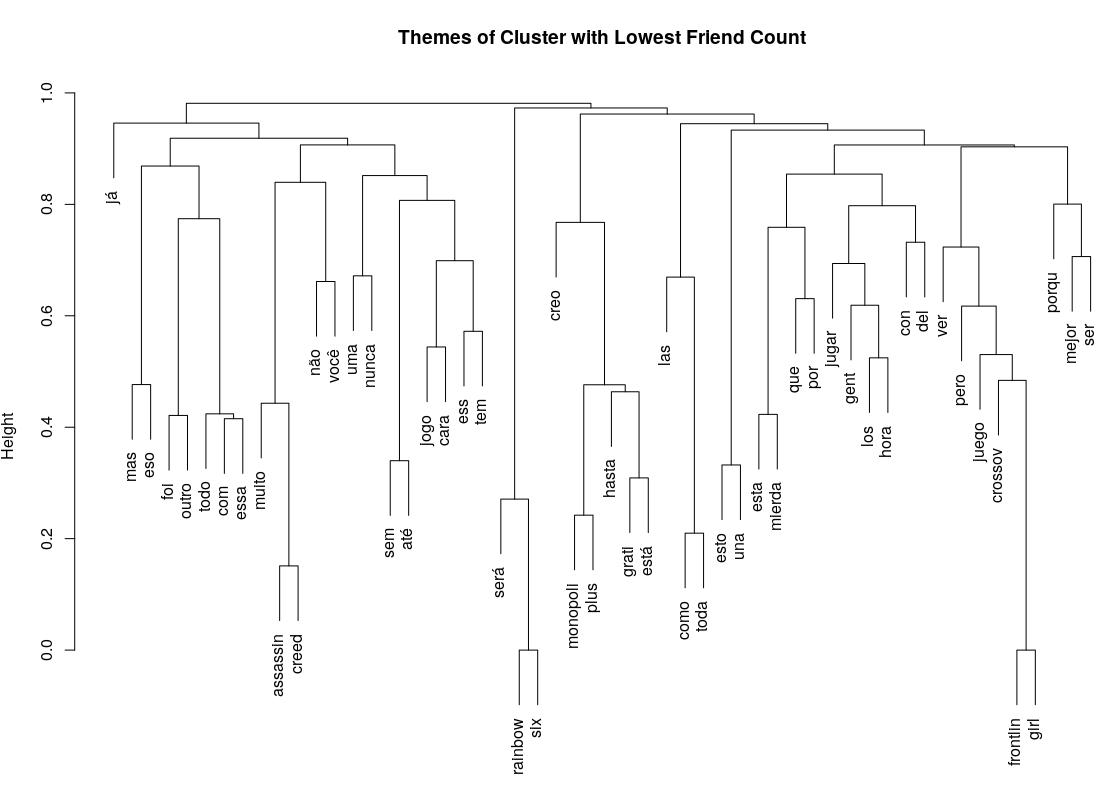
\includegraphics[width=12cm]{./Figures/LowDend.png}
\caption{\label{fig:org4715ef1}Dendrogram of Terms in the cluster with the highest friend count using average Linkage.}
\end{figure}

\subsection{8.2.23 Conclusion}
\label{sec:org482cd05}
It appears that users that discuss newer titles and upcoming collaborations belong to a cluster with a higher proportion of users with an above average friend count, whereas users that discuss older titles (such as \emph{Assasins Creed} as demonstrated in figure \ref{fig:org4715ef1}) tend to belong to a cluster with a lower proportion of users with high friend counts.

This could imply that users discussing new titles are more likely to have more friends or it could imply that twitter users with a high friend count are more likely to show interest in newer titles and material.
\section{Appendix}
\label{sec:org371a403}
\subsection{Users with High Friend Count}
\label{sec:org4d57598}

\begin{table}[htbp]
\caption{\label{tab:orgddeb848}User ID and Friend Count of users with above highest friend count in sample}
\centering
\begin{tabular}{rr}
\textbf{\emph{User ID}} & \textbf{\emph{Friend Count}}\\
\hline
274488119 & 8752\\
743771665 & 5002\\
1036014247 & 4999\\
2281452613 & 4992\\
1554453560 & 4958\\
981233818408570880 & 4944\\
931765564388921344 & 4836\\
807405140 & 4710\\
1112579152970842112 & 4514\\
2441577446 & 4322\\
552692862 & 4229\\
956297007127252992 & 3976\\
22493896 & 3675\\
255922782 & 3500\\
1067409881332936709 & 3312\\
27998570 & 3210\\
715118521555017728 & 3099\\
2356170174 & 2885\\
2372688230 & 2880\\
1868357425 & 2719\\
\end{tabular}
\end{table}
\subsection{Users with Low Friend Count}
\label{sec:org40946d2}
\begin{table}[htbp]
\caption{\label{tab:org41facb0}User ID and Friend Count of users with above highest friend count in sample}
\centering
\begin{tabular}{rr}
\textbf{\emph{User ID}} & \textbf{\emph{Friend Count}}\\
\hline
1254280995592966145 & 0\\
875126772978913280 & 0\\
1254256124217319425 & 0\\
1250219450210480128 & 0\\
1214921087328411648 & 0\\
1254115699628421120 & 0\\
1217600080376520704 & 0\\
1253480062453600257 & 0\\
1254178435502571521 & 0\\
1251955545092718592 & 0\\
1106864828700712960 & 0\\
1160744587620524032 & 0\\
1254256536710504448 & 1\\
1129040408384868352 & 1\\
1254121201871589376 & 1\\
1248687797755658243 & 2\\
1210265263867932675 & 2\\
3380784928 & 3\\
1177274165239275520 & 3\\
54645521 & 3\\
\end{tabular}
\end{table}

\subsection{TF-IDF Matrix}
\label{sec:orgb196e0d}

\begin{table}[htbp]
\caption{\label{tab:org36c1832}Document Term Matrix of first 6 documents and first 6 Words}
\centering
\begin{tabular}{rrrrrr}
\textbf{\textbf{check}} & \textbf{\textbf{coronavirus}} & \textbf{\textbf{death}} & \textbf{\textbf{first}} & \textbf{\textbf{gone}} & \textbf{\textbf{hour}}\\
\hline
0.615 & 0.747 & 0.830 & 0.596 & 0.747 & 0.698\\
0 & 0 & 0 & 0 & 0 & 0\\
0 & 0 & 0 & 0 & 0 & 0\\
0 & 0 & 0 & 0 & 0 & 0\\
0 & 0 & 0 & 0 & 0 & 0\\
0 & 0 & 0 & 0 & 0 & 0\\
\end{tabular}
\end{table}
\subsection{Relevant XKCD}
\label{sec:orgb7d6850}
\begin{figure}[htbp]
\centering
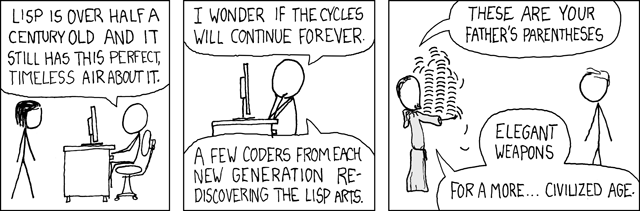
\includegraphics[width=7cm]{./Figures/lisp_cycles.png}
\caption{\label{fig:org84a8c26}\emph{xkcd} \texttt{\#} 297}
\end{figure}
\end{document}
